\chapter{Armonización}
\label{cap:armonizacion}



\section{¿Qué es armonizar?}
    \subsection{Pequeña introducción a la música}\label{sec:arm:armonia}

        Para entender lo explicado en posteriores secciones primero se hará en pequeño resumen de teoría musical. Vamos a definir la música como un conjunto de sonidos de duración variable organizados en el tiempo y que tienen cierto sentido estético, ya que pretenden transmitir emociones, ideas o belleza.

        Por lo tanto y, sintetizando al máximo, a nivel simbólico una canción la definen dos elementos: un conjunto de sonidos y un ritmo, es decir, la duración y el instante de tiempo en el que empieza cada sonido de ese conjunto. Nos centraremos por ahora en el primer elemento, ¿qué conjunto de sonidos se puede utilizar para componer una canción?
        Técnicamente cualquiera, al tratarse de una disciplina artística existe libre albedrío para realizar una composición. 

        \label{arm:notas_musicales}
        Sin embargo, nos centraremos en el estándar occidental, utilizado prácticamente en todas canciones que escuchuamos diariamente, en el que los sonidos se dividen en conjuntos de 12 notas musicales, cada una con un nombre diferente, difiniendo nota musical como un símbolo que representa una frecuencia determinada. Para entender de dónde viene esta división utilizaremos como base la nota A4 (La4), con una frecuencia de 440Hz y duplicaremos su frecuencia a 880Hz, obteniendo así A5 (La5). Estas dos notas comparten nombre, ya que si las escucháramos nos sonarían muy familiares entre sí. Esto tiene una explicación física: al reproducir esa frecuencia (frotando una cuerda, elevando una columna de aire...), no solo se genera la frecuencia fundamental, sino que también se producen armónicos, que son múltiplos enteros de la frecuencia fundamental. Se llama octava a la distancia que separa una frecuencia de su duplicación, esto explica ahora los número escritos al lado de cada nota musical: A3 = 220Hz, A4 = 440Hz, A5 = 880Hz. Sabiendo esto se decidió entonces dividir la octava en 12 notas musicales, perceptualmente equidistantes, la cual difiere con una equidistancia a nivel de frecuencia, debido a la naturaleza exponencial de las frecuencias. Es la llamada afinación temperada:

\begin{table}[h]
    \centering
    \begin{tabular}{c|c}
        \textbf{Nota Musical} & \textbf{Frecuencia (Hz)} \\
        \hline
        A4 & 440.00 \\
        A\#4 & 466.16 \\
        B4 & 493.88 \\
        C5 & 523.25 \\
        C\#5 & 554.37 \\
        D5 & 587.33 \\
        D\#5 & 622.25 \\
        E5 & 659.26 \\
        F5 & 698.46 \\
        F\#5 & 739.99 \\
        G5 & 783.99 \\
        G\#5 & 830.61 \\
        A5 & 880.00 \\
    \end{tabular}
    \caption{Tabla de Afinación Temperada de 12 Notas de A4 a A5}
    \label{tab:temperedTuningTable_A4_A5}
\end{table}

        Sacamos como conclusión que el conjunto de sonidos utilizados está comprendido por las 12 notas musicales, cada una puediéndose encontrar en una octava distinta. Hemos cambiado ligereamente la definición simbólica de canción entonces, pasando esta a estar compuestas por un ritmo y un conjunto de notas musicales (en vez de un conjunto de sonidos).  

        Así mismo, y entrando en otra capa de profundidad, ese conjunto de notas musicales que conformar una canción puede ser dividida en dos partes:

        \begin{enumerate}
            \item[\textbullet] \textbf{Melodía}: línea principal o motivo musical que guía la dirección y el desarrollo de una pieza musical. Parte más reconicible de una canción. En una composición musical es la que generalmente se canta o se toca de manera prominente.
            \item[\textbullet] \textbf{Armonía}: combinación simultánea de dos o más notas que se escuchan juntas y que suenan de manera agradable o consonante. La armonía proporciona un acompañamiento sonoro a la melodía principal y contribuye a enriquecer la textura musical. Se compone de acordes, que son grupos de notas tocadas simultáneamente.

        \end{enumerate}

    \subsection{Pequeña introducción a la armonía}

        Como se acaba de explicar, la armonía se define como la combinación y disposición de notas musicales que suenan de manera agradable y coherente entre sí. Para entender tanto la armonía, como los algoritmos que se quieren mostrar en este apartado del TFG, es necesario interiorizar los siguientes conceptos, que se intentarán explicar de la manera más resumida posible. Cabe recalcar que la explicación se realiza en el contexto de la armonía moderna, la cual difiere en algunos puntos de la clásica, sin embargo, al tratarse de una introducción, la mayoría de conceptos que van a ser mostrados se comparten entre ambas doctrinas. 

\begin{figure}[h]
    \centering
    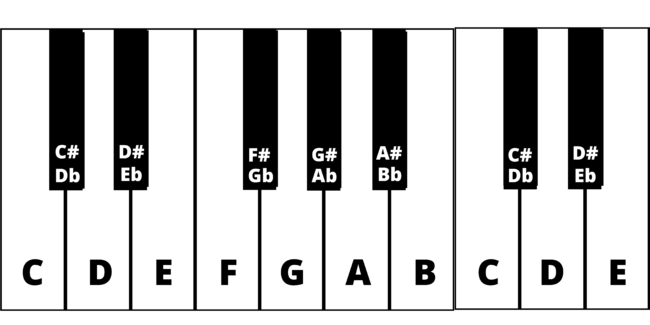
\includegraphics[width = 0.5\textwidth]{Imagenes/Bitmap/piano.png}
    \caption{Notas en el Piano}
    \label{fig:pianoImage}
\end{figure}

        \subsubsection{Intervalos}\label{sec:arm:intervalos}

        Un intervalo es la distancia que existe entre dos notas. Un semitono es la distancia mínima que puede existir entre dos notas. Un tono es igual a dos semitonos. Por ejemplo, en la figura \ref{fig:pianoImage} se puede observar que la distancia entre el primer C y el primer E es de 4 semitonos (las teclas negras también cuentan como notas musicales aunque tengan nombres un poco especiales). Podemos encontrar esa distancia mínima de un semitono entre C y C\# o entre E y F, por ejemplo. dependiendo del número de semitonos que tenga un intervalo, este tendrá un nombre y simbología diferente (también llamada grado en ciertos contextos que veremos posteriormente):

\begin{table}[h]
    \centering
    \begin{tabular}{c|c|c}
        \textbf{Símbolo (grado)} & \textbf{Nombre} & \textbf{Nº Semitonos} \\
        \hline
        1 (T) & Tónica & 0 \\
        b2 & Segunda menor & 1 \\
        2 & Segunda Mayor & 2 \\
        b3 & Tercera menor & 3 \\
        3 & Tercera Mayor & 4 \\
        4 & Cuarta Justa & 5 \\
        \#4 & Cuarta Aumentada & 6 \\
        5b & Quinta disminuida & 6 \\
        5 & Quinta Justa & 7 \\
        b6 & Sexta menor & 8 \\
        6 & Sexta Mayor & 9 \\
        b7 & Séptima menor & 10 \\
        7 & Séptima Mayor & 11 \\
        8 & Octava & 12 \\
    \end{tabular}
    \caption{Tabla de Intervalos}
    \label{tab:tabla_intervalos}
\end{table}

    Al observar la tabla se puede deducir por contexto que el símbolo 'b' (bemol) reduce en uno el número de semitonos del grado original, así como el símbolo 
    \# (sostenido) los aumenta en uno. Por ejemplo, \#6 sería equivalente a una séptima menor (b7), con 10 semitonos ambos. Así mismo estos símbolos se pueden apilar, por ejemplo, bb7 sería equivalente a uns sexta Mayor (6), con 9 semitonos ambos.

    Con la información de esta tabla, ya podríamos entender afirmaciones tales como 'la quinta Justa de C es G' o 'la tercera Mayor de B es D\#', por ejemplo, si nos ponemos a contar los semitonos más detenidamente.

    Cabe recalcar que, evidentemente existen intervalos que se salen de la octava, con más de 12 semitonos. Algunos no muy lejanos tienen incluso nombre propio, por ejemplo, una novena Mayor (9), de 14 semitonos. A pesar de ello, lo que se hará en estos casos es interpretar ese intervalo como su relativo si la nota estuviese en el 'mismo rango' que la tónica (nota desde la cual se mide el intervalo). Así, una novena Mayor sería equivalente a una segunda Mayor, de 2 semitonos y un intervalo de 42 semitonos será interpretado como una quinta disminuida (42 mod 12 = 6 semitonos), por ejemplo. De hecho, siguiendo esta definición, el propio intervalo de octava es redundante, ya que esta es equivalente a la tónica (12 mod 12 = 0 semitonos). Por ejemplo, la octava de C4 es C5. Por ello, el intervalo de octava también se debería quitar de la lista.

    \subsubsection{Escalas}\label{sec:arm:escalas}

    Se define escala como conjunto de 2 a 12 intervalos o grados ascencentes cuyo primer intervalo es siempre la tónica. Tradicionalmente, la mayoría de escalas están formadas por 7 grados, las más utilizadas en la música que escuchamos hoy en día son la Mayor y la menor.

\begin{table}[h]
    \centering
    \begin{tabular}{c|c|c|c|c|c|c|c}
        \textbf{Escala Mayor} & 1 (T) & 2 & 3 & 4 & 5 & 6 & 7 \\
        \hline
        \hline
        \textbf{Escala menor} & 1 (T) & 2 & b3 & 4 & 5 & b6 & b7 \\
    \end{tabular}
    \caption{Escalas Mayor y menor}
    \label{tab:escalas}
\end{table}

    Este conjunto de intervalos representa una espacie de esqueleto, un molde con el cual se puede crear una sucesión de notas musicales si se establece como tónica cualquiera de las 12 notas existentes. Aquí uno cuantos  ejemplos, utilizando como tónicas C, D y Bb:

\begin{table}[h]
    \centering
    \begin{tabular}{c|c|c|c|c|c|c|c}
        \textbf{C Mayor} & C (T) & D & E & F & G & A & B \\
        \hline
        \textbf{D Mayor} & D (T) & E & F\# & G & A & B & C\# \\
        \hline
        \textbf{Bb Mayor} & Bb (T) & C & D & Eb & F & G & A \\
        \hline
        \hline
        \textbf{C menor} & C (T) & D & Eb & F & G & Ab & Bb \\
        \hline
        \textbf{D menor} & D (T) & E & F & G & A & Bb & C \\
        \hline
        \textbf{Bb menor} & Bb (T) & C & Db & Eb & F & Gb & Ab \\
    \end{tabular}
    \caption{Escalas y Tónicas}
    \label{tab:escalas_tonicas}
\end{table}

    Para poner un poco más en contexto decir que, a parte de estas dos escalas, existen muchas otras más que se utilizan regularmente a la hora de componer música. Incluso existen compositores más vanguardistas que inventan nuevos conjuntos de grados, experimentando con nuevas formas de escribir música. Elgunos ejemplos: 

\begin{table}[h]
    \centering
    \begin{tabular}{c|c|c|c|c|c|c|c}       
        \textbf{pentatónica Mayor} & 1 (T) & 2 & 3 & 5 & \multicolumn{1}{c}{6} \\
        \hline
        \textbf{pentatónica menor} & 1 (T) & b3 & 4 & 5 & \multicolumn{1}{c}{b6} \\
        \hline
        \textbf{hexatónica} & 1 (T) & 2 & 3 & \#4 & \#5 & \multicolumn{1}{c}{\#6}  \\
        \hline
        \textbf{frigia} & 1 (T) & b2 & b3 & 4 & 5 & b6 & b7 \\
        \hline
        \textbf{mixolidia} & 1 (T) & 2 & 3 & 4 & 5 & 6 & b7 \\
        \hline
        \textbf{menor armónica} & 1 (T) & 2 & b3 & 4 & 5 & b6 & 7 \\      
    \end{tabular}
    \caption{Otras Escalas}
    \label{tab:otras_escalas}
\end{table}

    \subsubsection{Acordes}\label{sec:arm:acordes}

    Aunque no todo el mundo estaría de acuerdo con esta definición, vamos a decir que un acorde es un conjunto de dos o más notas tocadas de forma simultánea. La definición es en cierta medida similar a la de una escala, ya que un acorde no deja de ser un conjunto de intervalos ascendentes, en el que el primero es simpre la tónica del acorde. También se cumple esa propiedad de 'molde' a la hora de establecer una nota musical como tónica del acorde. Los acordes más comunes están formados por tres notas (triadas) y dependiendo del conjunto de intervalos se pueden conseguir diferentes sonoridades:

\begin{table}[h]
    \centering
    \begin{tabular}{c|c|c|c|c}       
        \textbf{Nombre} & \textbf{Símbolo} & \multicolumn{3}{c}{\textbf{Intervalos}} \\
        \hline
        \hline
        \textbf{Acorde Mayor} & & 1 (T) & 3 & 5 \\
        \hline
        \textbf{Acorde menor} & - & 1 (T) & b3 & 5 \\
        \hline
        \textbf{Acorde Aumentado} & + & 1 (T) & 3 & \#5 \\
        \hline
        \textbf{Acorde disminuido} & -b5 & 1 (T) & b3 & b5 \\
    \end{tabular}
    \caption{Triadas}
    \label{tab:triads}
\end{table}

\begin{table}[h]
    \centering
    \begin{tabular}{c|c|c|c|c}       
        \textbf{Nombre} & \textbf{Símbolo} & \multicolumn{3}{c}{\textbf{Notas}} \\
        \hline
        \hline
        \textbf{C Mayor} & C & C (T) & E & G \\
        \hline
        \textbf{C menor} & C- & C (T) & Eb & G \\
        \hline
        \textbf{C Aumentado} & C+ & C (T) & E & G\# \\
        \hline
        \textbf{C disminuido} & C-b5 & C (T) & Eb & Gb \\
    \end{tabular}
    \caption{Triadas en C}
    \label{tab:triadsC}
\end{table}

    \label{arm:armonia_escala}
    Se define como armonía de una escala el conjunto de acordes que se pueden formar utilizando únicamente las notas (o intervalos) de la escala. Esto puede chocar con la definición da acorde, ya que, como tal, puede haber miles de tipos acordes diferentes si atendemos a toda la combinatoria, así que, por ahora, solo tendremos en cuenta los tipos de acordes definidos anteriormente, es decir, acordes mayores, menores, aumentados y disminuidos. Este concepto es más difícil de deducir y explicar, así que recomiendo la visualización de \href{https://www.youtube.com/watch?v=dMwVB3BWcjI}{este vídeo} en el que el autor encuentra la armonía de la escala C Mayor y pasa el resultado a grados, además de repasar otros conceptos vistos por encima anteriormente. Se obtiene el siguiente resultado:

\begin{table}[h]
    \centering
    \begin{tabular}{c|c||c|c}
        \textbf{Grado} & \textbf{Acorde} & \textbf{Nota} & \textbf{Acorde} \\
        \hline
        1 (T) &  & C (T) & C \\
        2 & - & D & D- \\
        3 & - & E & E- \\
        4 &  & F & F \\
        5 &  & G & G \\
        6 & - & A & A- \\
        7 & -b5 & B & B-b5 \\
    \end{tabular}
    \caption{Tabla de Intervalos}
    \label{tab:tabla_intervalos}
\end{table}

    Como se puede observar, en la escala Mayor se forma una triada mayor a partir de los grados 1, 4 y 5, una menor a partir de los grados 2, 3 y 6, una disminuidoa a partir del grado 7 y no existe ningún grado del cual se forme una trida aumentada. Esto significa que sea cual sea la tónica de una escala, en este caso, la escala Mayor, los acordes correspondientes a cada grado serán siempre del mismo tipo. Por lo tanto, si se quiere deducir la armonía de una escala diferente, por ejemplo, la escala menor, los acordes correspondientes a cada grado serán distintos a los de la escala Mayor, pero serán del mismo tipo si se varía la tónica. Además, el hecho de que solo se forme un acorde por cada grado es debido a una particularidad propia de la escala Mayor y a que hemos escogido un número muy reducido de acordes. Vamos a tener en cuenta ahora el siguiente grupo de acordes de cuatro notas (cuatriadas), que se sumarán al anterior grupo:

\begin{table}[h]
    \centering
    \begin{tabular}{c|c|c|c|c|c}       
        \textbf{Nombre} & \textbf{Símbolo} & \multicolumn{4}{c}{\textbf{Intervalos}} \\
        \hline
        \hline
        \textbf{Acorde Mayor séptima} & maj7 & 1 (T) & 3 & 5 & 7\\
        \hline
        \textbf{Acorde de Dominante} & 7 & 1 (T) & 3 & 5 & b7\\
        \hline
        \textbf{Acorde menor séptima} & -7 & 1 (T) & b3 & 5 & b7 \\
        \hline
        \textbf{Acorde semidisminuido} & -7b5 & 1 (T) & b3 & b5 & b7 \\
        \hline
        \textbf{Acorde disminuido} & º & 1 (T) & b3 & b5 & bb7 \\
    \end{tabular}
    \caption{Cuatriadas}
    \label{tab:cuatriads}
\end{table}

    A continuación un par de ejemplos que evidencian el anterior párrafo: 

\begin{table}[h]
    \centering
    \begin{tabular}{c|c|c||c|c|c||c|c|c}
        \multicolumn{3}{c}{} & \multicolumn{3}{c}{\textbf{Escala Mayor}}  \\
        \hline  
        \multicolumn{1}{c|}{\textbf{Grados}} & \multicolumn{2}{c||}{\textbf{Acordes}} & \multicolumn{1}{c|}{\textbf{Notas}} & \multicolumn{2}{c||}{\textbf{Acordes}} & \multicolumn{1}{c|}{\textbf{Notas}} & \multicolumn{2}{c}{\textbf{Acordes}} \\
           \hline
    1 (T) &     & maj7 & C (T) & C    & Cmaj7 & D (T)   & D      & Dmaj7   \\
        2 & -   & -7   &    D  & D-   & D-7   &    E    & E-     & E-7     \\
        3 & -   & -7   &    E  & E-   & E-7   &    F\#  & F\#-   & F\#-7   \\
        4 &     & maj7 &    F  & F    & Fmaj7 &    G    & G      & Gmaj7   \\
        5 &     & 7    &    G  & G    & G7    &    A    & A      & A7      \\
        6 & -   & -7   &    A  & A-   & A-7   &    B    & B-     & B-7     \\
        7 & -b5 & -7b5 &    B  & B-b5 & B-7b5 &    C\#  & C\#-b5 & C\#-7b5 \\
        \hline
        \multicolumn{3}{c}{} & \multicolumn{3}{c}{\textbf{Escala menor}}  \\
        \hline  
        \multicolumn{1}{c|}{\textbf{Grados}} & \multicolumn{2}{c||}{\textbf{Acordes}} & \multicolumn{1}{c|}{\textbf{Notas}} & \multicolumn{2}{c||}{\textbf{Acordes}} & \multicolumn{1}{c|}{\textbf{Notas}} & \multicolumn{2}{c}{\textbf{Acordes}} \\
           \hline 
    1 (T)  & -   & -7   & C (T)  & C-    & C-7    & D (T) & D-   & D-7    \\
        2  & -b5 & -7b5 &    D   & Db-b5 & Db-7b5 &    E  & E-b5 & E-7b5  \\
        b3 &     & maj7 &    Eb  & E     & Emaj7  &    F  & F    & Fmaj7  \\
        4  & -   & -7   &    F   & F-    & F-7    &    G  & G-   & G-7    \\
        5  & -   & -7   &    G   & G-    & G-7    &    A  & A-   & A-7    \\
        b6 &     & maj7 &    Ab  & Ab    & Abmaj7 &    Bb & Bb   & Bbmaj7 \\
        b7 &     & 7    &    Bb  & Bb    & Bb7    &    C  & C    & C7     \\

    \end{tabular}
    \caption{Comparativa entre Escalas (Mayor y menor) y Tónicas (C y D)}
    \label{tab:comparativa_scalas}
\end{table}
    

    Todo lo mostrado hasta ahora forma parte de las bases de composición musical. Básicamente escoger una escala y una tónica, y utilizar todo el conjunto de notas y acordes que se forman a partir de estas para crear una melodía y una armonía (un acompañamiento). Sin embargo, esto es solo la punta del iceberg, ya que si se prfundiza, se podrán descubrir otros conceptos, como la modulación (cambio de tonalidad), el uso de acordes y notas de otras escalas, la libertad para salirse de las restricciones de la escala establecida, etc. 

\subsection{Cuestión a resolver}     

    Una vez que se conoce todo este contexto ya se puede presentar el problema que se pretende abordar en esta sección o módulo de la aplicación: dada una melodía cualquiera, encontrar la armonía que mejor se adapte a esta, es decir, buscar la mejor secuencia de acordes que acompañen y enriquezcan a la melodía. Esta secuencia de acordes sería utilizada por posteriores módulos de la aplicación.

    Cabe dejar claro que, buscar 'la mejor' armonía para una melodía es algo relativo, ya que depende de la subjetividad de cada persona. Así que lo dejaremos en buscar una armonía fuertemente coherente para una melodía dada, que forme parte del espectro de soluciones razonables, ya que, por lo general, una melodía puede ser acompañada por varios conjuntos de acordes distintos.

    También comentar que, al resolver este problema, se estaría construyendo de forma implícita un analizador armánico. Si la entrada a este módulo fuese, en vez de únicamente una melodía, una canción completa, la cual contiene mucha más información, la salida esparada sería la armonía de dicha canción. Esto tiene mucha utilidad, ya que el análisis armónico es fundamental para el estudio en profundidad de una obra. La armonía son los cimientos de una composición musical. 

    \section{Técnicas de armonización utilizadas}

    Antes de empezar con las técnicas de armonización utilizadas, falta un paso previo crucial. Y es la creación de una estructura de clases y métodos que den soporte a todo lo explicado en el apartado \ref{sec:arm:armonia}. Existe una clases que abstraen lo que representa una \hyperref[arm:notas_musicales]{\textcolor{blue}{nota musical}}, un \hyperref[sec:arm:intervalos]{\textcolor{blue}{intervalo}}, una \hyperref[sec:arm:escalas]{\textcolor{blue}{escala}} y la \hyperref[arm:armonia_escala]{\textcolor{blue}{armonía de una escala}} tal como se ha explicado. Un \hyperref[sec:arm:acordes]{\textcolor{blue}{acorde}} es respresentado también como una escala. 
    
    También es importante mostrar las respresentaciones que se están utilizando para almacenar una canción (conjunto de notas) en este módulo de la aplicación. Existen métodos para pasar de la primera representación a la segunda:

    \begin{enumerate}
        \item \textbf{Lista de Notas}: es la representación estándar en este módulo de la aplicación. Se almacenan de forma desordenada diccionarios con la siguiente estructura:
        \begin{enumerate}
            \item[\textbullet] \textbf{note}: almacena el pitch (tono) de la nota. Guardar el pitch es similar a guardar la nota musical, ya que este almacena de forma implícita el nombre de la nota y su octava. Por ejemplo, calculemos a qué nota le corresponde el pitch 40:
            \begin{enumerate}
                    \item[\(\circ\)] \textbf{Nombre}: 40 mod 12 = 4, según la tabla \ref{tab:nota_pitch} a un 4 le corresponde E
                    \item[\(\circ\)] \textbf{Octava}: 40 div 12 = 3, está en la tercera octava
            \end{enumerate}
                       
\begin{table}[htbp]
    \centering
    \begin{tabular}{c|c}
        \textbf{Nombre} & \textbf{Pitch} \\
        \hline
        C & 0 \\
        C\# / Db & 1 \\
        D & 2 \\
        D\# / Eb & 3 \\
        E & 4 \\
        F & 5 \\
        F\# / Gb & 6 \\
        G & 7 \\
        G\# / Ab & 8 \\
        A & 9 \\
        A\# / Bb & 10 \\
        B & 11 \\
    \end{tabular}
    \caption{Relación entre cada Nota Musical y su Pitch en la Primera Octava}
\label{tab:nota_pitch}
\end{table}

        \item[\textbullet] \textbf{start\_time}: tiempo en ticks en el que empieza a sonar una nota desde que empieza la canción en el tick 0
        \item[\textbullet] \textbf{duartion}: tiempo en ticks desde que empieza a sonar la nota hasta que para
    \end{enumerate}
    \item \textbf{Diccionario de Ticks}: se almacena en cada tick clave el evento que ha ocurrido. Los ticks clave están ordenados de menor a mayor. Como tal, solo existen dos tipos de eventos: 
    \begin{enumerate}
        \item[\textbullet] \textbf{note\_on}
        \item[\textbullet] \textbf{note\_off}
    \end{enumerate}
    A cada evento viene asociado el pitch de la nota afectada. Esto puede suponer, a priori, un inconveniente, ya que, si hay dos notas del mismo pitch superpuestas en el mismo espacio de tiempo, existe una ambigüedad a la hora de saber qué evento note\_off le corresponde a cada una. Sin embargo, esta representación se utiliza de forma temporal para facilitar la implementación de ciertos algoritmos a los cuales cuales este inconveniente no les afecta. 
    
\end{enumerate}

    Falta por explicar el concepto de tick. Un tick es la unidad simbólica mínima e indivisible que puede durar una nota. En cada canción (conjunto de notas) se debe definir el número de ticks que dura un pulso. Un pulso también se puede traducir como una negra, un beat o un step. Cuanto mayor sea el número de ticks por pulso, mayor será el número de partes en el que puedes dividir el pulse. Haciendo una analogía con la representación simbólica que se utiliza en las partituras, si los ticks por pulso son iguales a 4, en nuestra canción la semicorchea sería la representación mínima que se podría utilizar, mientras que si fueran igual a 8, la fusa sería la representación mínima (una fusa es la mitad de una semicorchea). De todas formas, lo normal es que los el número de ticks por pulso sea más alto para permitir mayor número de divisiones y combinaciones.

    


    